\chapter{Posterior Regularization}
Posterior regularization is an alternative way of clustering the phrases.
Unlike a Baysian approach where intuitions about the data are expressed through the priors, posterior regularization imposes constraints on posterior distributions of the data.

In this chapter , we will introduce a basic clustering model with EM 
and look at shortcomings of the basic model. This will motivate us for
more complicated posterior regularized models.
\section{Phrase Clustering Model} 
As a brief recap, the clustering problem we are working with
is to label phrases with $K$ induced categories, where
$K$ is picked manually.
Phrases are obtained from bi-text data.
We also look at context
 words before and after
phrases as cues for clustering.
The relationship between phrases, contexts and categories are
represented with a generative model shown in 
Figure \ref{fig:EM}: a phrase picks a 
category and then that category generates the contex for the phrase.

\begin{figure}[h]
  \centering
  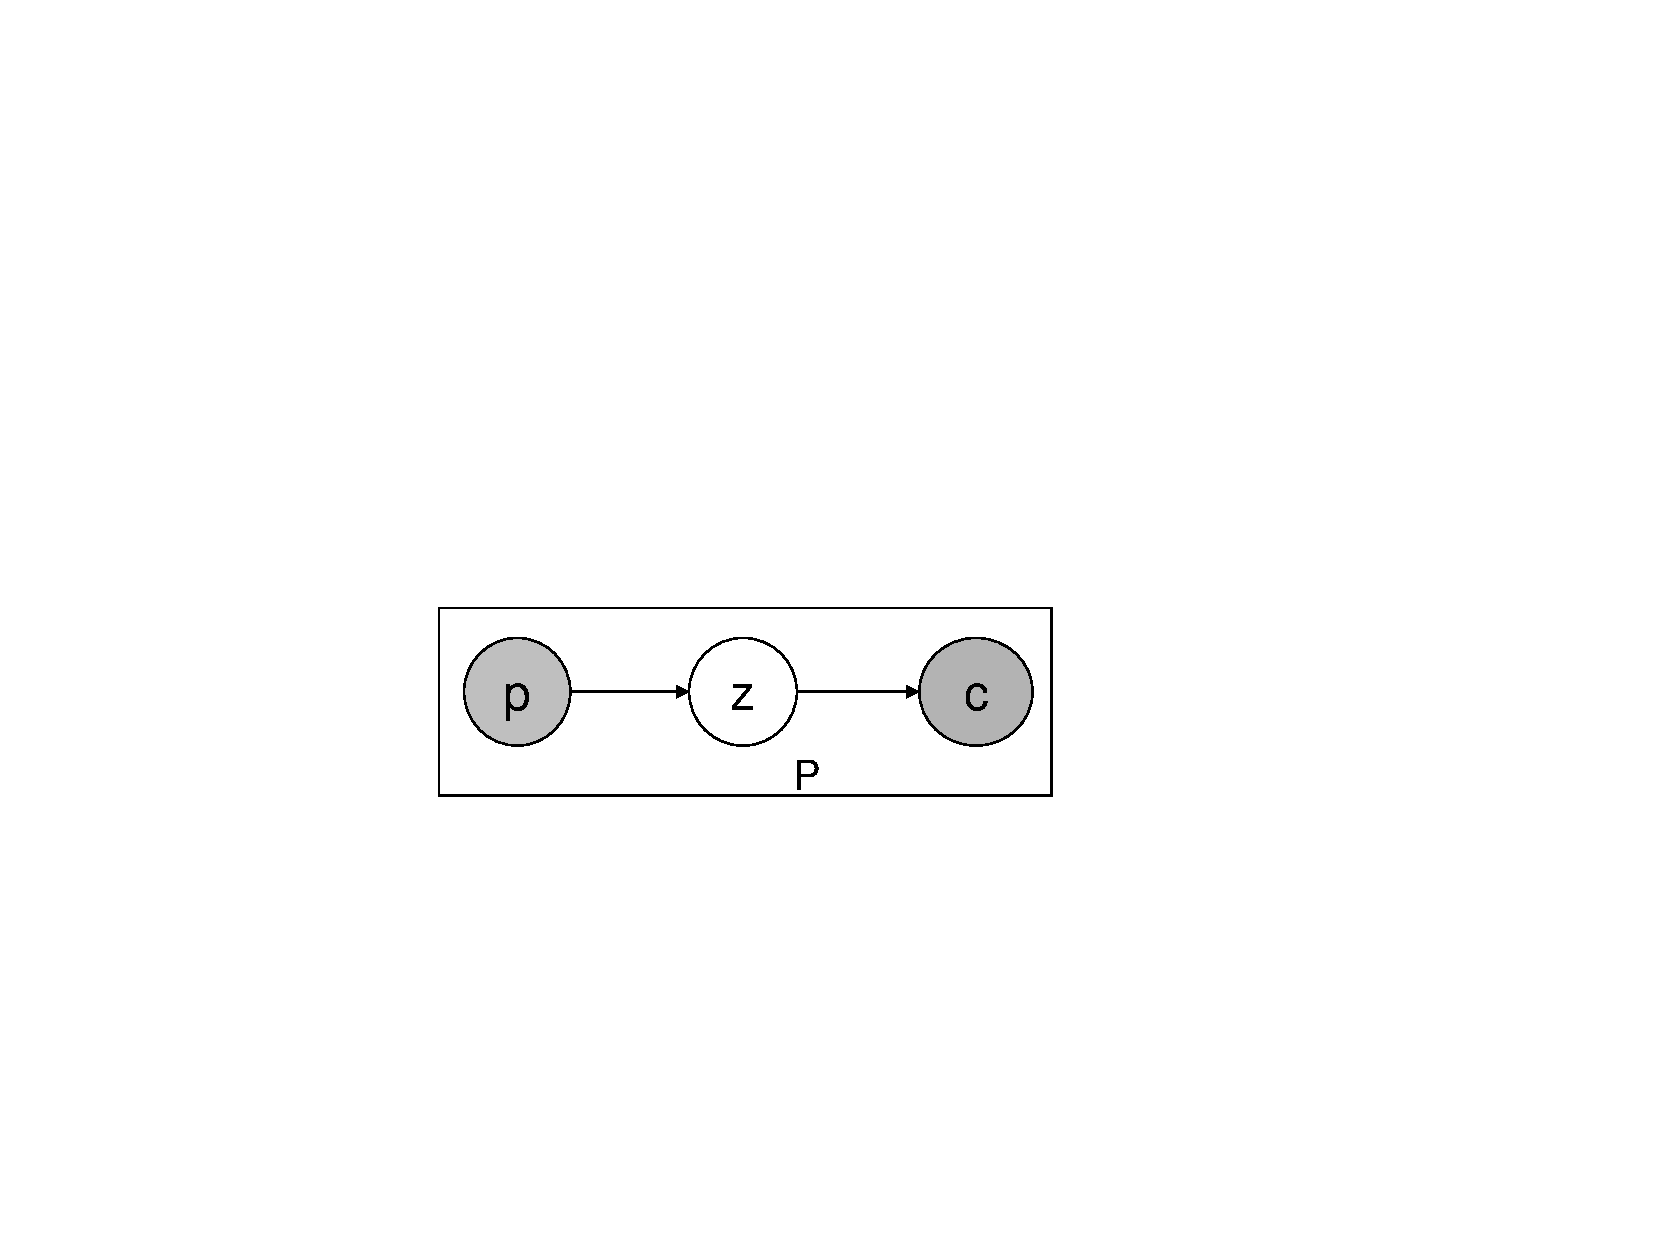
\includegraphics[width=3.0in]{pr-clustering/EMdigram}
  \caption{Basic Phrase Clustering Model}
  \label{fig:EM}
\end{figure}

The joint probability of a category $z$ and a context $\textbf{c}$ 
given a phrase $\textbf{p}$ is
\[
P(z,\textbf{c}|\textbf{p})=P(z|\textbf{p})P(\textbf{c}|z).
\]
$P(z|\textbf{p})$ is distribution of categories given a phrase.
This can be learned from data.
$P(\textbf{c}|z)$ is distribution of context given a category.
Since a context usually contains multiple slots for words, we further
decompose this distribution into independent distributions at
each slot. For example, suppose a context consists of two positions 
before and after the phrase. Denote these words as 
$c_{-2},c_{-1},c_1,c_2$.
Use $P_{-2},P_{-1},P_1,P_2$ to denote distributions of words at each 
position, $P(\textbf{c}|z)$ is decomposed as
\[
P(\textbf{c}|z)=P_{-2}(c_{-2}|z)P_{-1}
(c_{-1}|z)P_1(c_1|z)P_2(c_2|z).
\]
The posterior probability of a category given a phrase
and a context can be computed by normalizing the joint probability:
\[
P(z|\textbf{p},\textbf{c})=\frac{P(z,\textbf{c}|\textbf{p})}
{\sum_{i=1,K}P(i,\textbf{c}|\textbf{p})}.
\]
With the mechanisms to compute the posterior probabilities, we can 
apply EM to learn all the probabilities.
\section{Sparsity Constraints}
A common linguistic intuition we have about the phrase 
clustering problem is that a phrase should be put into very
few categories, e.g. a verb phrase is unlikely to be used as 
a noun phrase. In other words, the categorization of
a phrase should be sparse.
The generative model we proposed above with EM
allows a phrase to be labelled with many tags. As we observed
from the output, EM is using more categories than we wanted for
each phrase.
Posterior regularization
provides a way to enforce sparsity \citep{ganchev:penn:2009}.
The general idea of posterior regularization is to modify
E-step of EM, so that instead of using posterior distribution
as the $q$ distribution directly, we want to find the nearest
$q$
in a constrained space  as shown in Figure \ref{fig:EMPR}.

\begin{figure}[h]
  \centering
  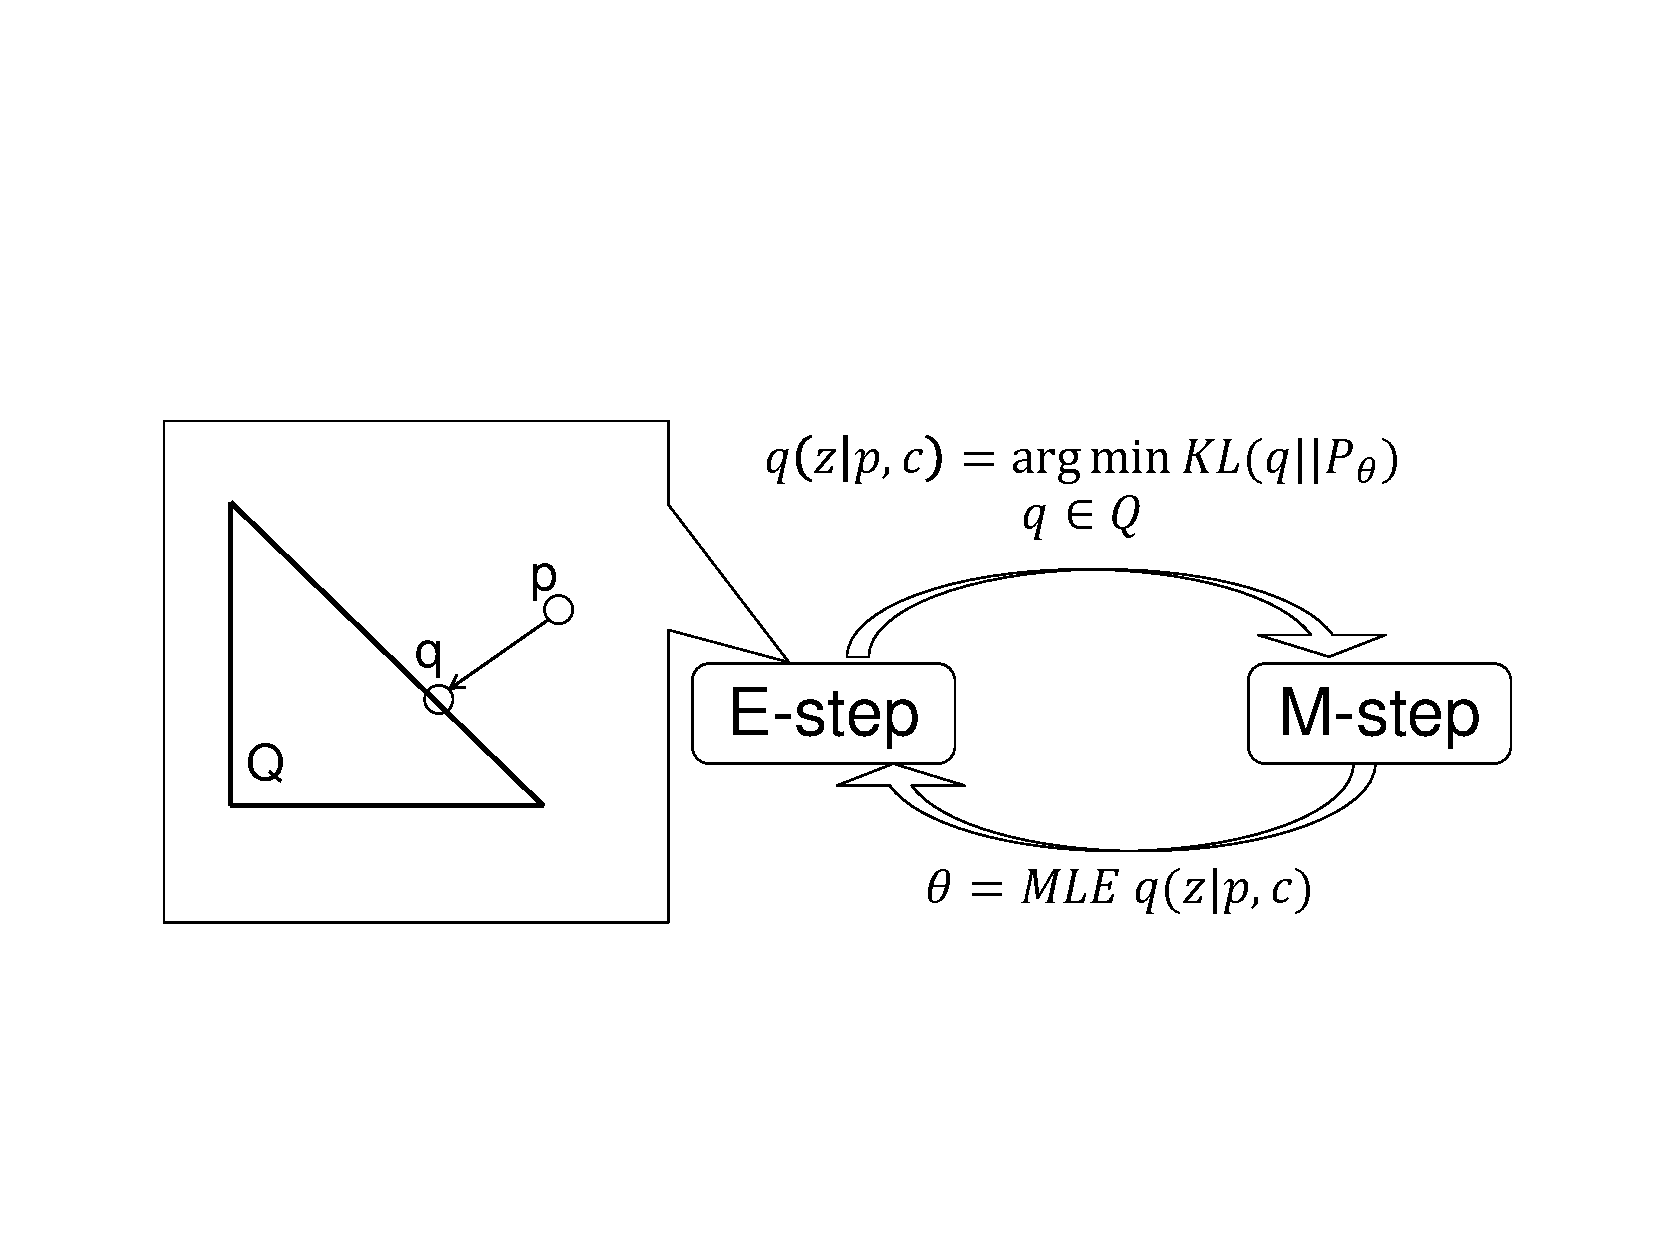
\includegraphics[width=3.5in]{pr-clustering/EMPR}
  \caption{EM with posterior regularization}
  \label{fig:EMPR}
\end{figure}

The constraint we use here is called $l_1/ l_\infty$
regularization in Ganchev's technical report. The notations
we use here largely follows Ganchev's.
In a more mathematical formulation, for each phrase $\textbf{p}$,
we want the quantity 
\[\sum_{z=1}^K \max_i P(z|\textbf{p},\textbf{c}_i) \]
to be small, where $\textbf{c}_i$ is the context
appeared around the $i$th occurrence of phrase $\textbf{p}$
throughout the data. This quantity roughly equals 
the number of categories phrase $\textbf{p}$ uses.
It is minimized to $1$ if and only if
the posterior distributions $P(z|\textbf{p},\textbf{c}_i)$
are the same
for all
occurrences of $\textbf{p}$. That is ,
$\forall i,j$, $P(z|\textbf{p},\textbf{c}_i)=P(z|\textbf{p},\textbf{c}_j)$. 

Define feature functions for $i$th occurrence of phrase $\textbf{p}$
with category $j$,
as a function of category $z$:
\[
\phi_{\textbf{p}ij}(z)=
\begin{cases}
1\text{ if z=j}\\
0\text{ otherwise}
\end{cases}.
\]
For notation simplicity, for
each phrase category pair, 
define variables $c_{\textbf{p}z}$ that will
eventually be $\max_i E_q[\phi_{\textbf{p}iz}]$.
The objective we want to optimize becomes:
\[
\arg\min_{q,c_{\textbf{p}z}} KL(q||P_{\theta}) + 
\sigma \sum_{\textbf{p},z}c_{\textbf{p}z}
\]
\[
\text{ s.t. }\forall \textbf{p},z,
E_q[\phi_{\textbf{p}iz}]\leq c_{\textbf{p}z}.
\]
Using Lagrange Multipliers, this objective can
be optimized in its dual form,
for each phrase $\textbf{p}$:
\[
\arg\min_{\lambda\geq 0} \log 
(\sum_{z,i} P_\theta(z|\textbf{p},\textbf{c}_i)
\exp (-\lambda_{\textbf{p}iz}))
\]
\[
\text{ s.t. } \forall \textbf{p},z,
\sum_i \lambda_{\textbf{p}iz}\leq \sigma.
\]
This dual objective can be optimized with projected gradient
descent.
The $q$ distribution we are looking for is then
\[
q_i(z)\propto P_{\theta}(z|\textbf{p},\textbf{c}_i)
\exp(\lambda_{\textbf{p}iz}).
\]
M-step can be performed as usual.
\section{Agreement Models}
Another type of constraint we used is agreement between
different models. We came up with a similar generative
model in the reverse direction to agree with 
as shown in Figure \ref{fig:EMreverse}. We also
took advantage of bi-text data we have and make models
learning from different languages agree with each other.

\begin{figure}[h]
  \centering
  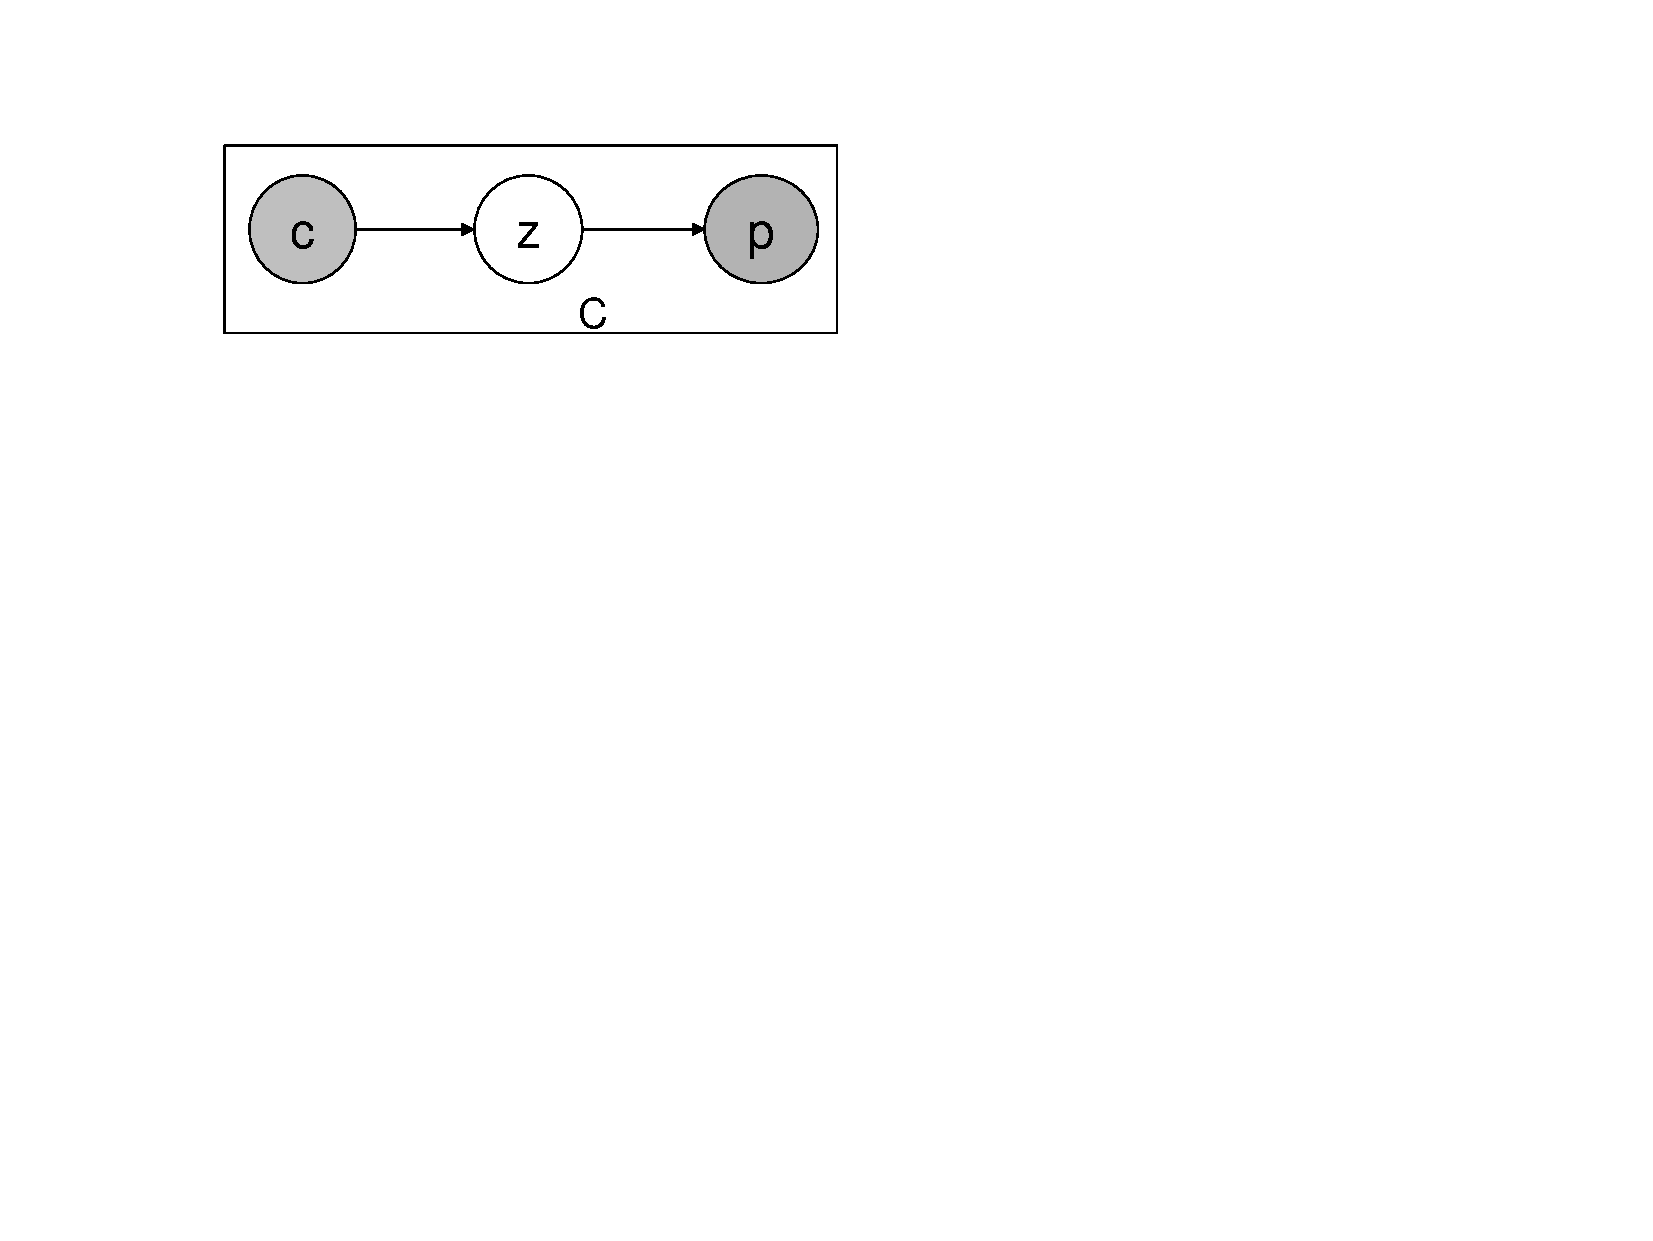
\includegraphics[width=3.0in]{pr-clustering/EMreverse}
  \caption{EM with posterior regularization}
  \label{fig:EMreverse}
\end{figure}

In the reversed model,
the posterior probability of the labelling of
a context $\textbf{c}$ with
phrase $\textbf{p}$ is 
\[
P(z|\textbf{c},\textbf{p})\propto 
P(z|\textbf{c})P(\textbf{p}|z).
\]
Since a phrase contains a variable number of words,
we only look at the first and last word of
a phrase. That is $P(\textbf{p}|z)=P_1(p_1|z)P_n(p_n|z)$,
where $n$ is the length of $\textbf{p}$, $P_1$ and $P_n$
denotes distributions for words in the first and last position
of a phrase given a category.

The implementation of agreement models again ends up making
a small change to E-step. The $q$ distribution for
a phrase $\textbf{p}$ and a context $\textbf{c}$ 
is given by
\[
q(z)=\sqrt{P_{\theta 1}
(z|\textbf{p},\textbf{c})P_{\theta 2}(z|\textbf{p},\textbf{c})},
\]
where $P_{\theta 1}$ and $P_{\theta 2}$ are
posterior distributions for two models.
In M-step, both models should update their parameters with the
same $q$ distribution computed as above.
This modified EM maximizes the objective:
\[
\mathcal{L}_1+
\mathcal{L}_2+
\sum_{\textbf{p},\textbf{c}}
\log\sum_z\sqrt{P_{\theta 1}(z|\textbf{p},\textbf{c})
P_{\theta 2}(z|\textbf{p},\textbf{c})},
\]
where $\mathcal{L}_1$ and $\mathcal{L}_2$
are log-likelihood of
two models.
\section{Experiments}
